% SPDX-License-Identifier: LPPL-1.3c
% Copyright (C) 2026 Christophe Jorssen
% Author and Current Maintainer: Christophe Jorssen <christophe.jorssen@gmail.com>
% LPPL maintenance status: maintained
% This file is part of luafemm. See LICENSE and LICENSES.md for its terms.
\section{Drawing eddy-current loops and splitting a conductor}
\label{sec:currents}

For real time snapshots, the same pic displays the instantaneous induced current;
no harmonic phase is applied. Section~\ref{sec:time} gives a switched-current
example and a loss history. The axial H formulation below remains harmonic.

\subsection{Which plane contains the current?}
A current plot must respect the direction of the computed current.
Before choosing arrows or symbols, identify the drawing plane. In an ordinary planar magnetic problem,
$\mathbf B$ lies in the page and $J_z$ points through it. In an axisymmetric
$(r,z)$ section, the current is azimuthal: its circles also leave that page.
Neither picture contains in-plane current streamlines.

The |femm eddy currents| pic chooses a physical view of the current:
\begin{itemize}
\item |view=symbols| draws dots and crosses for currents out of and into the
page. This is the automatic view of planar and axisymmetric models.
\item |view=loops| draws an axisymmetric body's actual circular currents in a
separate transverse $(x,y)$ section, at a specified axial position.
\item |view=lines| traces computed transverse streamlines in the new
|type=axial| diffusion model. Here $B_z$ points through the page, and
$\mathbf J$ circulates within it. This is that model's automatic view.
\end{itemize}
The last model is especially useful for comparing a solid cylinder with an
insulated bundle under the axial field of a long solenoid. It is a different
reduction of Maxwell's equations, not a rotated axisymmetric drawing.
No general three-dimensional streamline tracer is implied.

\subsection{A cylinder, nineteen rods and one exciting coil}
Consider a copper cylinder of radius $R$ inside a long coil of radius
$R+\varepsilon$. The coil imposes an axial sinusoidal field. Viewed along the
cylinder axis, the section is a circle. Declare the imposed \emph{magnetic}
field rather than an out-of-page current source:
\begin{codeexample}[code only]
\tikzset{induction experiment/.style={
  femm/problem={type=axial,frequency=50,applied field=.01,
    depth=100,xmin=-8,xmax=8,ymin=-8,ymax=8,mesh size=.65}}}
% In a picture with this style:
\filldraw[fill=gray!25,
  femm/region={material=copper,mesh size=.24,curve tolerance=.002}]
  (0,0) circle[radius=6];
\pic[femm/currents={phase=90,lines=6}] {femm eddy currents};
\end{codeexample}
The peak field in the surrounding insulator is $B_0=0.01\,\mathrm T$ and
$f=50\,\mathrm{Hz}$. A depth of $100$ means $100\,\mathrm{mm}$ with the default
unit. It converts per-length energy and loss into totals; it does not introduce
finite-length end effects. The long-solenoid excitation corresponds to
$n\widehat I=B_0/\mu_0$, with $n$ the number of turns per unit length.
The drawn coil circle identifies its radius. It is not a meshed circuit or a
computed finite coil. This approximation prescribes $H_z$ in the connected
insulator and neglects displacement current.

Replace the solid section by $N$ circular conductors of radius
$a=R/\sqrt N$. Their total copper area remains
$N\pi a^2=\pi R^2$. The rods are electrically separated by insulation, so each
has its own closed current loops. The illustrated $N=19$ packing has one
central rod, six on the first ring and twelve on the second, as in the supplied
lamination sketch. The example exposes |\Radius|, |\Strands|, |\Gap|,
|\Epsilon|, |\Frequency|, |\AppliedB| and |\Length| as ordinary TeX parameters.
Its explicit packing accepts integer $1\leq N\leq19$; other packings can be
written with ordinary TikZ paths and loops without changing the solver.

There is a geometric catch: the bundle's enclosing radius is \emph{larger}
than $R$. Insulating gaps and packing voids occupy additional area. One cannot
retain both the same metal area and the same radius-$R$ envelope. The example
uses the same coil radius in both pictures and checks that the bundle fits.
For the nineteen-rod packing, its outer ring has radius
\[
 d=2a+g,\qquad \rho_2=\frac{d}{2\sin15^\circ},\qquad
 R_{\rm envelope}=\rho_2+a,
\]
where $g$ is the minimum gap within each ring. The alternating angular offset
keeps the two rings separated. With $R=6\,\mathrm{mm}$, $g=0.12\,\mathrm{mm}$
and $\varepsilon=1.5\,\mathrm{mm}$, both specimens fit in the
$7.5\,\mathrm{mm}$ coil. Increasing $N$ or the gap may require a larger coil.
The computational rectangle must also contain every physical region.

\subsection{Measure the effect instead of counting arrows}
Each picture chooses its contour levels independently. Six current lines per
rod do not mean that the rods carry the same current density as the solid
cylinder. Register a radial profile and measure the copper losses:
\begin{codeexample}[code only]
% Declare this profile while the solid-cylinder model is current:
\path[femm/profile={name=solid-radius,samples=81}] (0,0)--(5.994,0);
\femmselect[name=solid-metal,material=copper]
\femmmeasure[name=solid-loss,selection=solid-metal]
% Later, in a PGFPlots axis:
\femmplot[profile=solid-radius,component=Jn,abscissa=t,
  representation=rms,plot options={blue,thick}]
\end{codeexample}
On a profile running along the positive $x$ radius, its left normal is the
positive azimuthal direction, so |Jn| is $J_\theta$. The complete example stops
at $0.999a$, just inside the conductor, and rescales the plotted abscissa to
$r/a$ with a PGFPlots |x filter|. This avoids the ambiguous triangle choice
exactly on a metal--air interface, where current density is discontinuous.
The derivative of a P1 field is piecewise constant; steps in a current profile
are a visible discretisation effect. More sample points alone do not remove
them. Start with a coarse mesh when arranging the figure, then reduce local
|mesh size| relative to both the rod radius and the skin depth, and refine
|curve tolerance| before comparing losses.

In the weak-skin limit, a nonmagnetic circular conductor has
\[
 \widehat J_\theta(r)\simeq-\frac{\mathrm i\omega\sigma B_0r}{2},\qquad
 \frac{P(a)}{L}\simeq\frac{\pi\sigma\omega^2B_0^2a^4}{16}.
\]
Consequently $P_N/P_1\simeq1/N$ at equal total metal area. This is a limiting
law, not an imposed numerical scaling: the solver computes each geometry's
shielding and currents. As skin effects grow, the ratio need not be $1/N$.
For the stated copper parameters the computed ratio is about $0.053$, close
to $1/19\simeq0.0526$. The complete source prints its own solved losses and
ratio, and plots the two RMS current profiles on a common scale.
\luafemmexamplebegin{eddy-current-bundle}

% manual example: eddy-current-bundle/1

\begin{codeexample}[setup code]
\def\Radius{6}\def\Strands{19}\def\Gap{.12}\def\Epsilon{1.5}
\def\Frequency{50}\def\AppliedB{.01}\def\Length{100}
\pgfmathsetmacro{\RodRadius}{\Radius/sqrt(\Strands)}
\pgfmathsetmacro{\Pitch}{2*\RodRadius+\Gap}
\pgfmathsetmacro{\OuterRing}{\Pitch/(2*sin(15))}
\pgfmathsetmacro{\CoilRadius}{\Radius+\Epsilon}
\pgfmathsetmacro{\Envelope}{\RodRadius+(\Strands>7 ? \OuterRing : (\Strands>1 ? \Pitch : 0))}
\ifnum\Strands<1 \errmessage{Strands must be between 1 and 19}\fi
\ifnum\Strands>19 \errmessage{This example packing supports at most 19 strands}\fi
\ifdim\Envelope pt>\CoilRadius pt \errmessage{Increase Epsilon to fit the insulated bundle}\fi
\tikzset{axial induction/.style={femm/problem={type=axial,
    frequency=\Frequency,applied field=\AppliedB,depth=\Length,
    xmin=-8,xmax=8,ymin=-8,ymax=8,mesh size=.65},scale=3,
    femm/arrow spacing=7mm,femm/arrow length=1mm,femm/arrow width=.65mm},
  metal/.style={draw=black!65,fill=gray!25,
    femm/region={material=copper,mesh size=\MetalMesh,curve tolerance=.002}},
  exciting coil/.style={draw=blue!65!black,dashed,thick}}
\pgfmathsetmacro{\MetalMesh}{\Radius/25}
\end{codeexample}

The following picture uses the preceding definitions.

% manual example: eddy-current-bundle/2

\begin{codeexample}[width=0pt]
\begin{tikzpicture}[axial induction,femm/cache={file=\jobname-solid,mode=auto}]
  \fill[gray!7] (0,0) circle[radius=\CoilRadius];
  \filldraw[metal] (0,0) circle[radius=\Radius];
  \draw[exciting coil] (0,0) circle[radius=\CoilRadius];
  \path[femm/profile={name=solid-radius,samples=81}] (0,0)--({.999*\Radius},0);
  \pic[femm/currents={phase=90,lines=6}] {femm eddy currents};
  \femmselect[name=solid-metal,material=copper]
  \femmmeasure[name=solid-loss,selection=solid-metal]
  \node[above] at (0,8) {One solid cylinder, radius $R$};
  \node[below] at (0,-8) {$P_1=\femmvalue[component=joule_loss,
    number format={sci,precision=3}]{solid-loss}$};
\end{tikzpicture}
\end{codeexample}

% manual example: eddy-current-bundle/3

\begin{codeexample}[setup code]
\pgfmathsetmacro{\MetalMesh}{\RodRadius/15}
\end{codeexample}

The following picture uses the preceding definitions.

% manual example: eddy-current-bundle/4

\begin{codeexample}[width=0pt]
\begin{tikzpicture}[axial induction,femm/cache={file=\jobname-bundle,mode=auto}]
  \fill[gray!7] (0,0) circle[radius=\CoilRadius];
  \foreach \i in {1,...,\Strands}{
    \ifnum\i=1
      \def\CentreRadius{0}\def\Angle{0}
    \else\ifnum\i<8
      \let\CentreRadius\Pitch\pgfmathsetmacro{\Angle}{60*(\i-2)}
    \else
      \let\CentreRadius\OuterRing\pgfmathsetmacro{\Angle}{15+30*(\i-8)}
    \fi\fi
    \filldraw[metal] (\Angle:\CentreRadius) circle[radius=\RodRadius];
  }
  \draw[exciting coil] (0,0) circle[radius=\CoilRadius];
  \path[femm/profile={name=rod-radius,samples=81}] (0,0)--({.999*\RodRadius},0);
  \pic[femm/currents={phase=90,lines=6}] {femm eddy currents};
  \femmselect[name=bundle-metal,material=copper]
  \femmmeasure[name=bundle-loss,selection=bundle-metal]
  \node[above] at (0,8) {$N=\Strands$ isolated rods, $a=R/\sqrt N$};
  \node[below] at (0,-8) {$P_N=\femmvalue[component=joule_loss,
    number format={sci,precision=3}]{bundle-loss}$};
\end{tikzpicture}
\end{codeexample}

% manual example: eddy-current-bundle/5

\begin{codeexample}[width=0pt]
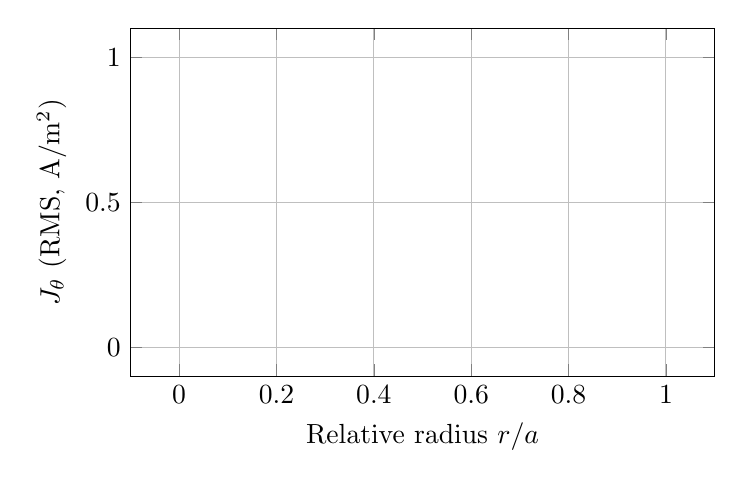
\begin{tikzpicture}
\begin{axis}[width=9cm,height=6cm,grid=major,no markers,
    xlabel={Relative radius $r/a$},ylabel={$J_\theta$ (RMS, $\mathrm{A/m^2}$)},
    legend pos=north west,
    x filter/.code={\pgfmathparse{.999*#1}}]
  \femmplot[profile=solid-radius,component=Jn,abscissa=t,representation=rms,
    plot options={blue!65!black,thick}]
  \addlegendentry{Solid cylinder}
  \femmplot[profile=rod-radius,component=Jn,abscissa=t,representation=rms,
    plot options={red!70!black,thick}]
  \addlegendentry{Central isolated rod}
\end{axis}
\end{tikzpicture}
\end{codeexample}

\luafemmexampleend{eddy-current-bundle}

\subsection{Showing the circles of an axisymmetric current}
A conducting tube inside a finite solenoid is a different useful example.
Keep |type=axisymmetric|, where the finite coil is an actual winding source.
A first pic marks the induced current through the meridional page. A second
pic draws its circular loops at |section=0|, displaced to the right for clarity:
\begin{codeexample}[code only]
\pic[femm/currents={view=symbols,spacing=1.5,phase=90}]
  {femm eddy currents};
\pic[femm/currents={view=loops,section=0,center x=55,
  spacing=.6,phase=90},femm/arrow spacing=10mm]
  {femm eddy currents};
\end{codeexample}
Here $+J_\varphi$ points \emph{into} the $(r,z)$ page, so it is a cross there;
it runs anticlockwise in the transverse $(x,y)$ view. A positive planar $J_z$
is a dot. Both views use the same solved phasors and the same time phase.
The winding is stranded and is not included in the eddy-current glyphs.
\luafemmexamplebegin{eddy-current-views}

% manual example: eddy-current-views/1

\begin{codeexample}[width=0pt]
\begin{tikzpicture}[femm/problem={type=axisymmetric,frequency=1000,
    xmax=30,ymin=-25,ymax=25,mesh size=2},
    femm/circuit={name=drive,current=2},
    femm/cache={file=\jobname,mode=auto},scale=1.2]
  \filldraw[fill=orange!20,draw=orange!70!black,
    femm/region={material=copper,circuit=drive,turns=100,mesh size=1}]
    (12,-12) rectangle (16,12);
  \filldraw[fill=gray!25,draw=gray,
    femm/region={material=copper,mesh size=.5}]
    (5,-10) rectangle (8,10);
  \pic[femm/currents={view=symbols,spacing=1.5,phase=90},
    femm/eddy style={color=red!70!black}] {femm eddy currents};
  \draw[dashed] (0,-25)--(0,25) node[above] {$z$};
  \draw[dashed,blue!60!black] (0,0)--(25,0) node[right] {$z=0$};
  \node[above] at (15,26) {Meridional section $(r,z)$};

  \fill[gray!25,even odd rule] (55,0) circle[radius=8] (55,0) circle[radius=5];
  \draw[gray] (55,0) circle[radius=8] (55,0) circle[radius=5];
  \pic[femm/currents={view=loops,section=0,center x=55,spacing=.6,phase=90},
    femm/arrow spacing=10mm] {femm eddy currents};
  \node[above] at (55,12) {Transverse section $(x,y)$};
  \node[below] at (55,-12) {$\omega t=90^\circ$};
\end{tikzpicture}
\end{codeexample}

\luafemmexampleend{eddy-current-views}

\subsection{Problem keys and the order of operations}
Declare |femm/problem| first, followed by materials and all physical regions.
Register profiles and selections. Then request a current pic, a measurement or
a plot; each solves on demand. After meshing, do not add or alter physical
regions. Use a new problem for another specimen or frequency. Any number of
current pics may choose independent phases and styles without recomputation.

\begin{key}{/femm/problem/type=axial}
Select the transverse long-conductor $H_z$ formulation. |planar| remains the
default; |axisymmetric| means a meridional $A_\varphi$ model instead.
Axial mode requires positive |frequency| and |mesher=delaunay| (the default
mesher). Arbitrary simply connected solid-conductor cross-sections and several
separated conductors are supported. Their surrounding nonconducting material
must have relative permeability one and remain connected to the exterior.
An insulating cavity enclosed by metal has an unknown coupled axial field and
is rejected. Excluded holes are also rejected; draw insulating regions when
appropriate. Real isotropic linear conductive materials are accepted; nonlinear
laws, coercivity, anisotropy and catalogue loss/lamination/wire models are not.

This mode has passive conductors only: impressed current densities, stranded
regions, named winding circuits, specialised boundaries, ideal circuits and
planar component nodes are unavailable. The scalar conductor-surface condition
is imposed automatically. Standard vector-potential boundary values must stay
at their defaults. Public FEM/ANS interchange does not represent this model;
use its native cache and the TikZ source. Ordinary TikZ curve capture, material
styles and local mesh controls remain available.
\end{key}
\begin{key}{/femm/problem/applied field=\meta{tesla} (initially .01)}
Signed peak axial flux-density amplitude in the surrounding insulator, for
|type=axial|. It sets $\widehat H_0=(B_0/\mu_0)e^{\mathrm i\alpha}$.
Zero is allowed and yields zero field and current. This is a physical source,
not a plotting scale. It has no effect on planar or axisymmetric models.
\end{key}
\begin{key}{/femm/problem/applied phase=\meta{degrees} (initially 0)}
Phase $\alpha$ of the imposed axial field, with the harmonic
$e^{+\mathrm i\omega t}$ convention. Source amplitude and phase enter the
physical cache fingerprint. They are distinct from the current pic's time phase.
\end{key}

\subsection{Current-pic keys and styles}
\begin{key}{/tikz/femm/currents=\marg{options}}
Set the following |/femm/currents| keys. Apply the key to a |tikzpicture| or
scope for shared defaults, or to a pic for local overrides. It is a normal
PGF key family and can be included in reusable |.style| definitions.
\end{key}
\begin{key}{/femm/currents/view=\meta{choice} (initially auto)}
A |.is choice| handler accepting |auto|, |lines|, |symbols| and |loops|.
Automatic selection follows the formulation as explained above. Incompatible
views raise an error; planar scalar currents are never reinterpreted as
in-plane vectors. Only induced currents in solid conductors are drawn.
\end{key}
\begin{key}{/femm/currents/phase=\meta{degrees} (initially 90)}
Instantaneous time phase $\omega t$. A quarter-period default makes weak-skin
currents readily visible under a phase-zero imposed cosine field. It is
independent of |/tikz/femm/phase| and the profile's |phase| (both initially zero).
\end{key}
\begin{key}{/femm/currents/material=\meta{name} (initially empty)}
Restrict the view to a declared material. Empty means all conductive materials;
unknown names raise an error. Use distinct material names when specimens need
independent selection even though their properties coincide.
\end{key}
\begin{key}{/femm/currents/lines=\meta{integer} (initially 7)}
For |view=lines|, choose 1 to 200 equally spaced interior streamfunction levels
between the selected conductors' extrema. A level may produce several closed
paths, one in each rod. This does not specify a line count per connected body
or an absolute current increment. Zero current produces no paths.
\end{key}
\begin{key}{/femm/currents/spacing=\meta{model units} (initially 2)}
Positive target spacing of symbol centres or sampled loop radii. The bounds
are divided into equally sized cells no larger than this spacing, with samples
at their centres. Only centres in conducting material are drawn. Thin regions
can be missed by a coarse grid; reduce spacing to resolve them. This controls
the display only, not the field mesh. Symbol grids above 10000 cells and radial
loop grids above 1000 cells are rejected. |view=lines| ignores this key.
\end{key}
\begin{key}{/femm/currents/section=\meta{model units} (initially 0)}
Axial coordinate $z$ of a transverse |view=loops| section, within the model's
vertical bounds. Each radius is sampled in the original meridional solution.
\end{key}
\begin{key}{/femm/currents/center x=\meta{model units} (initially 0)}
\end{key}
\begin{key}{/femm/currents/center y=\meta{model units} (initially 0)}
Drawing centre of the transverse loop view, expressed in the problem's root
coordinate frame. These keys move its illustration, not the physical solution
or the sampled section. Other views ignore them. Like field pics, current pics
use the root problem transform; a local pic shift does not move solved geometry.
\end{key}
\begin{key}{/femm/currents/reference current=\meta{amperes per square metre} (initially 0)}
For symbols and loops, zero chooses the largest sampled absolute instantaneous
current density. A positive value sets an explicit common opacity reference
for comparison across pics. Relative strength $q=\min(1,|J|/J_{\rm ref})$
gives opacity $0.2+0.8q$. Sign controls direction; opacity encodes magnitude.
The key does not affect |view=lines|, whose paths have unit opacity.
\end{key}
\begin{key}{/femm/currents/minimum fraction=\meta{number} (initially .02)}
Suppress symbols and loops with $q$ at or below this threshold. The accepted
range is $0\leq q_{\min}<1$. This avoids drawing numerical near-zero currents
with arbitrary direction. |view=lines| ignores the threshold.
\end{key}
\begin{key}{/femm/currents/symbol radius=\meta{TeX dimension} (initially 1.3pt)}
Radius of each dot/cross circle, in physical page units. Model scaling affects
its position, not this radius. Keep the dimension positive.
\end{key}
\begin{key}{/tikz/femm/eddy style=\marg{TikZ options}}
Append local drawing options after the base |femm eddy line| or
|femm eddy symbol| style. The defaults use a fine dark-red stroke and the
existing oriented-field arrows. |femm/arrows|, |femm/arrow spacing|,
|femm/arrow length| and |femm/arrow width| also apply to current paths.
Set colours and line patterns with ordinary TikZ styles:
\begin{codeexample}[code only]
\tikzset{induced loops/.style={femm/currents={phase=90,lines=8},
  femm/eddy style={blue!65!black,line width=.4pt},femm/arrow spacing=8mm}}
\pic[induced loops] {femm eddy currents};
\end{codeexample}
\end{key}

\subsection{Profiles, losses and the discrete formulation}
Axial profiles add |Bz| and |Hz|, and the transverse current components
|Jx|, |Jy|, |Jt| and |Jn|. The last two project onto the oriented profile's
unit tangent and left normal. Current units are $\mathrm{A/m^2}$.
|J| and |Jeddy| coincide and mean the vector norm in axial mode; they remain
signed out-of-page scalars in planar/axisymmetric mode. A vector norm has no
single phase: request |phase| on a signed component instead. All usual harmonic
representations work. In-plane magnetic components are zero; |B| and |H|
are the norms of the axial field. Vector-potential and meridional-flux
components are unavailable. The |femm field| pic is rejected because its
in-plane magnetic contours would have no physical meaning in this model.

Regional measurements supply |area|, |volume|, |energy|, |coenergy|,
|joule_loss| and |eddy_loss|. The two losses coincide; energy and coenergy
are equal cycle averages. Supply positive |depth| for totals. Current integrals
and forces are unavailable in this reduction. Losses use
$\int(|\widehat J_x|^2+|\widehat J_y|^2)/(2\sigma)\,dV$ and need no graphical
contour or glyph sampling.

In a conductive domain, the weak form is
\[
 \int\frac1\sigma\nabla\widehat H_z\mathbin{\cdot}\nabla v\,dS
 +\mathrm i\omega\int\mu\widehat H_zv\,dS=0,
 \qquad \widehat H_z|_{\partial\Omega}=\widehat H_0,
 \qquad \widehat{\mathbf J}=(\partial_y\widehat H_z,-\partial_x\widehat H_z).
\]
The implementation stores the dimensionless P1 perturbation
$u=\widehat H_z/\widehat H_0-1$ and solves its unit-drive equation even when
$B_0=0$, then multiplies physical fields by the requested source. The same
complex ILU(0)--GMRES solver and consistent mass used for harmonic magnetics
apply. Internally named |A| arrays contain this perturbation in axial mode;
they must never be exported or interpreted as vector potential. Use
|luafemm-harmonic.sample| for phasors and the public profile/measurement keys.
Cache format 24 distinguishes the formulation, source and both scalar arrays.

At a fixed phase, the $H_z$ contours are current streamlines, with orientation
from $(\partial_yH_z,-\partial_xH_z)$. Constant surface $H_z$ makes the normal
current vanish on conductor boundaries. P1 interpolation yields continuous
streamfunction contours and piecewise constant currents. The cylinder benchmark
compares against
\[
 \widehat H_z(r)=\widehat H_0\frac{I_0(kr)}{I_0(ka)},\qquad
 \widehat J_\theta(r)=-\widehat H_0 k\frac{I_1(kr)}{I_0(ka)},\qquad
 k=\frac{1+\mathrm i}{\delta}.
\]
The tests evaluate the modified Bessel functions independently by power series,
check mesh convergence and Joule losses, then test equal-area insulated disks,
closed loop orientation, cache restoration and all three generic TeX formats.
They do not validate finite-cylinder end effects or inter-strand contact.
